\documentclass{article}
\title{TDSC Episode 1: How Much Does a Polar Bear Weigh?}
\author{Michael Rosenburg \\ Narain Krishnamurthy \\ Ian Quah}
\usepackage{amsmath}
\usepackage{amsfonts}
\usepackage{courier}
\usepackage{turnstile}
\usepackage{blkarray}
\usepackage{enumerate}
\usepackage{hyperref}
\usepackage{graphicx}
\graphicspath{ {/Users/narainsk/Documents/15418/assignment2/} }
\makeatletter
\newbox\BA@first@box
\def\@seccntformat#1{%
  \expandafter\ifx\csname c@#1\endcsname\c@section\else
  \csname the#1\endcsname\quad
  \fi}
\makeatother
\begin{document}
\maketitle

<<<<<<< HEAD
\section{Techniques}
We were interested in using longitude and latitude to predict the number of
subscriber users in a given area, to predict whether or not a female user
was more likely to rent a bike from a given area, and to predict whether or
not a non-subscriber was going to renta  bike from a given area. To handle these
issues, we chose to implement a kernel regression for each bike station, where
we chose to regress number of subscriber users who used a given station on the
longitude and latitude coordinates of that station. In order to handle the
categorical outcomes related to female and non-subscriber users, we chose to
use decision trees of these outcomes on the trip duration, birth year of the
user, and the longitude and latitude coordinates of the bike rental station.
We then pruned these decision trees using a five-fold cross-validation method.

\section{Results}
See plots for our results. We found that the number of subscriber users were
maximized in our kernel regression at longitude-latitude range $(-74,40.74
-40.76).$ We see that the general division line where we are more likely to
see a woman user is above and at the latitude of $40.748$. We see that the
optimal longitude and latitude for seeing a non-subscriber user is below
the longitude bound of $-73.98$, and below the latitude point of $40.76$.
We found that, based on the outcomes of the decision
trees and the kernel regression, the optimal locations that satisfied both
our categorical outcomes and maximizing the number of users was at
longitude-latitude coordinates $(-74, 40.76)$ and $(-74, 40.74)$.

\end{document}
=======
\section{Overview}
We 

\section{Model Description}
asdf

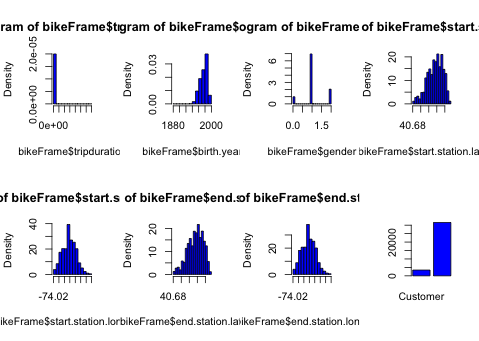
\includegraphics[scale=0.5]{EDA.png}

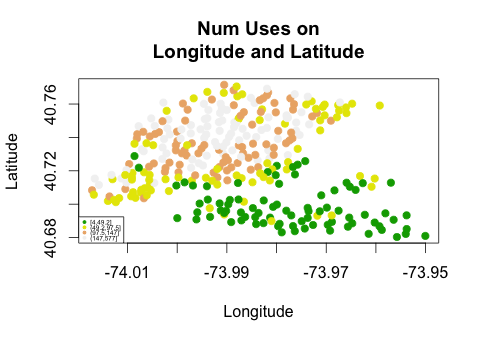
\includegraphics[scale=0.5]{num_uses.png}

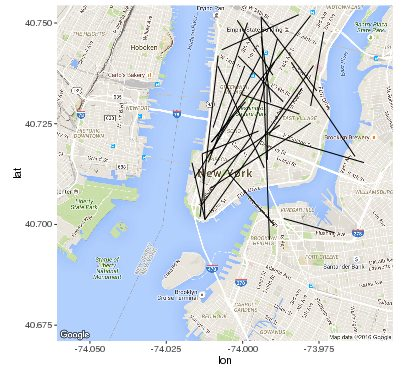
\includegraphics[scale=1.0]{female_most_traficked_routes.jpg}

\end{document}
>>>>>>> 255743817f27b20815bfa47f825af1546fe93d8e
